%%%%%%%%%%%%%%%%%%%%%%%%%%%%%%%%%%%%%%%%%%%%%%%%%%%%%%%%%%%%%%%%
%%                          CHAPTER 2                         %%
%%%%%%%%%%%%%%%%%%%%%%%%%%%%%%%%%%%%%%%%%%%%%%%%%%%%%%%%%%%%%%%%
\chapter{The synchroniser compiler}
  \section{Mathematical Model}
Synchroniser $S = (\Phi, \; \Pi)$, where
  \begin{itemize}
  \item[] $\Phi = (A, \; S, \; T)$ -- nondeterministic state machine:
    \begin{itemize}
    \item[] $A \subseteq C \times P$ -- the alphabet of events, $C$ -- set of synchroniser input channels, $P$ -- set of predicates on channel messages. An event $(c, \; p) \in A$ represents the reception of a message on channel $c$ that satisfies predicate $p$,
    \item[] $S \supseteq \{s_{0}\}$ -- set of abstract states, $s_{0}$ -- start state,
    \item[] $T \: : \: A \times S \to S$ -- transition matrix.
    \end{itemize}
  \item[] $\Pi \: : \: S \times \Omega \to V$ -- path functional that defines the synchroniser output:
    \begin{itemize}
    \item[] $\Omega$ -- the set of output channels,
    \item[] $V$ -- the set of message values \cite{astrakahn}.
    \end{itemize}
  \end{itemize}

In a state $s_{k}$ the functional is based on the retrospective sequence of transitions from the most recent visit to the start state $s_{0}$ to $s_{k}$:
  \begin{itemize}
  \item[] $(s_{0}, c_{0}), \: (s_{1}, c_{1}),... \: (s_{k}, c_{k})$, where
    \begin{itemize}
      \item[] $s_{0}$ -- start state,
      \item[] $c_{i} \in C$, $0 \le i \le k$ -- the channel that caused the transition from the state $s_{i}$.
    \end{itemize}
  \end{itemize}

Let $\mu_{i}$ be the message received in the transition from the state $s_{i}$. Then
  \begin{itemize}
  \item[] $\Pi \; (s_{k}, \omega_{m}) = \psi_{\sqcap} \; \{\mu_{i} \: | \: \rho_{ki}^{m} \; (s_{i}), \: 0 \le i \le k\}$, where
    \begin{itemize}
      \item[] $\rho_{ki}^{m}$ -- selection predicate that defines $\Pi$,
      \item[] $\psi_{\sqcap}$ -- the operator that coerces the messages in the operand set to their joint greatest subtype.
    \end{itemize}
  \end{itemize}

From the above, the synchroniser is fully defined by two functions:
  \begin{enumerate}
  \item The transition matrix $T$

The state machine can have a regular structure whereby many transitions can be defined at once by a formula with some limited range integer variables. For example, a machine with 8 states could have a transition matrix defined thus: $S_{k \; mod \; 8} \to S_{k+1 \; mod \; 8}$.

In order to be able to use regular structures, \ak\ allows synchronisers to declare \emph{state} variables.

\textbf{Example: the counter synchroniser}  Counter emits every $n$-th message received in its input channel to the output channel. The transition diagram for the counter synchroniser for $n = 3$ is given in Figure \ref{fig:counter}.a.

Mathematical model $S_{counter_{3}} = (\Phi, \; \Pi)$, where
  \begin{itemize}
  \item[] $\Phi = (A, \; S, \; T)$,
    \begin{itemize}
    \item[] $C = (a)$, $P = (true)$, $A = C \times P = ((a, \; true))$,
    \item[] $S = (s_{0}, \; s_{1}, \; s_{2})$, $s_{0}$ -- start state,
    \item[] $T$:
      \begin{tabular}{c|c|c|c}
      $A$ \textbackslash $S$ & $s_{0}$ & $s_{1}$ & $s_{2}$\\
      \hline
      $(a, \; true)$ & $s_{1}$ & $s_{2}$ & $s_{0}$\\
      \end{tabular}
    \end{itemize}
  \item[] $\Pi \: : \: S \times \Omega \to V$,
    \begin{itemize}
    \item[] $\Omega = (c)$,
    \item[] $V = (a)$
    \end{itemize}
  \end{itemize}

An output message is emitted when a transition happens from the state $s_{2}$. This state is reached in a single path:
  \begin{itemize}
  \item[]
$W_{0} = ((s_{0}, \; a), \: (s_{1}, \; a), \: (s_{2}, \; a))$
% fixed rho{1i}^{c} to rho{2i}^{c}
$\Pi \; (s_{2}, c) = \psi_{\sqcap} \; \{\mu_{0} = a \: | \: \rho_{20}^{c} \; (s_{0}) = 0, \mu_{1} = a \: | \: \rho_{21}^{c} \; (s_{1}) = 0, \mu_{2} = a \: | \: \rho_{22}^{c} \; (s_{2}) = 1\}$, $k = 1$, $i = 0,1,2$ 
  \end{itemize}

The state machine behind the counter has a regular structure, and for this synchroniser all its transitions may be defined with a single formula: $S_{k \; mod \; 3} \to S_{k+1 \; mod \; 3}$. Considering this, the transition matrix $T$ would be:
  \begin{tabular}{c|c}
  $A$ \textbackslash $S$ & $S_{k \; mod \; 3}$\\
  \hline
  $(a, \; true)$ & $S_{k+1 \; mod \; 3}$
  \end{tabular}

Some possible transition diagrams of the counter synchroniser are given in Figure \ref{fig:counter}. The diagram \ref{fig:counter}.a represents the unrolled regular structure of the synchroniser. However, this representation is inconvenient when $n \gg 1$. The transition diagram \ref{fig:counter}.a can be folded using state variables. Two possible variants are shown in figures \ref{fig:counter}.b and \ref{fig:counter}.c. The state variable $c$ acts as an induction variable in a while loop with the exit condition $c \ge 3$.

  \begin{figure}[here]
  \centering
  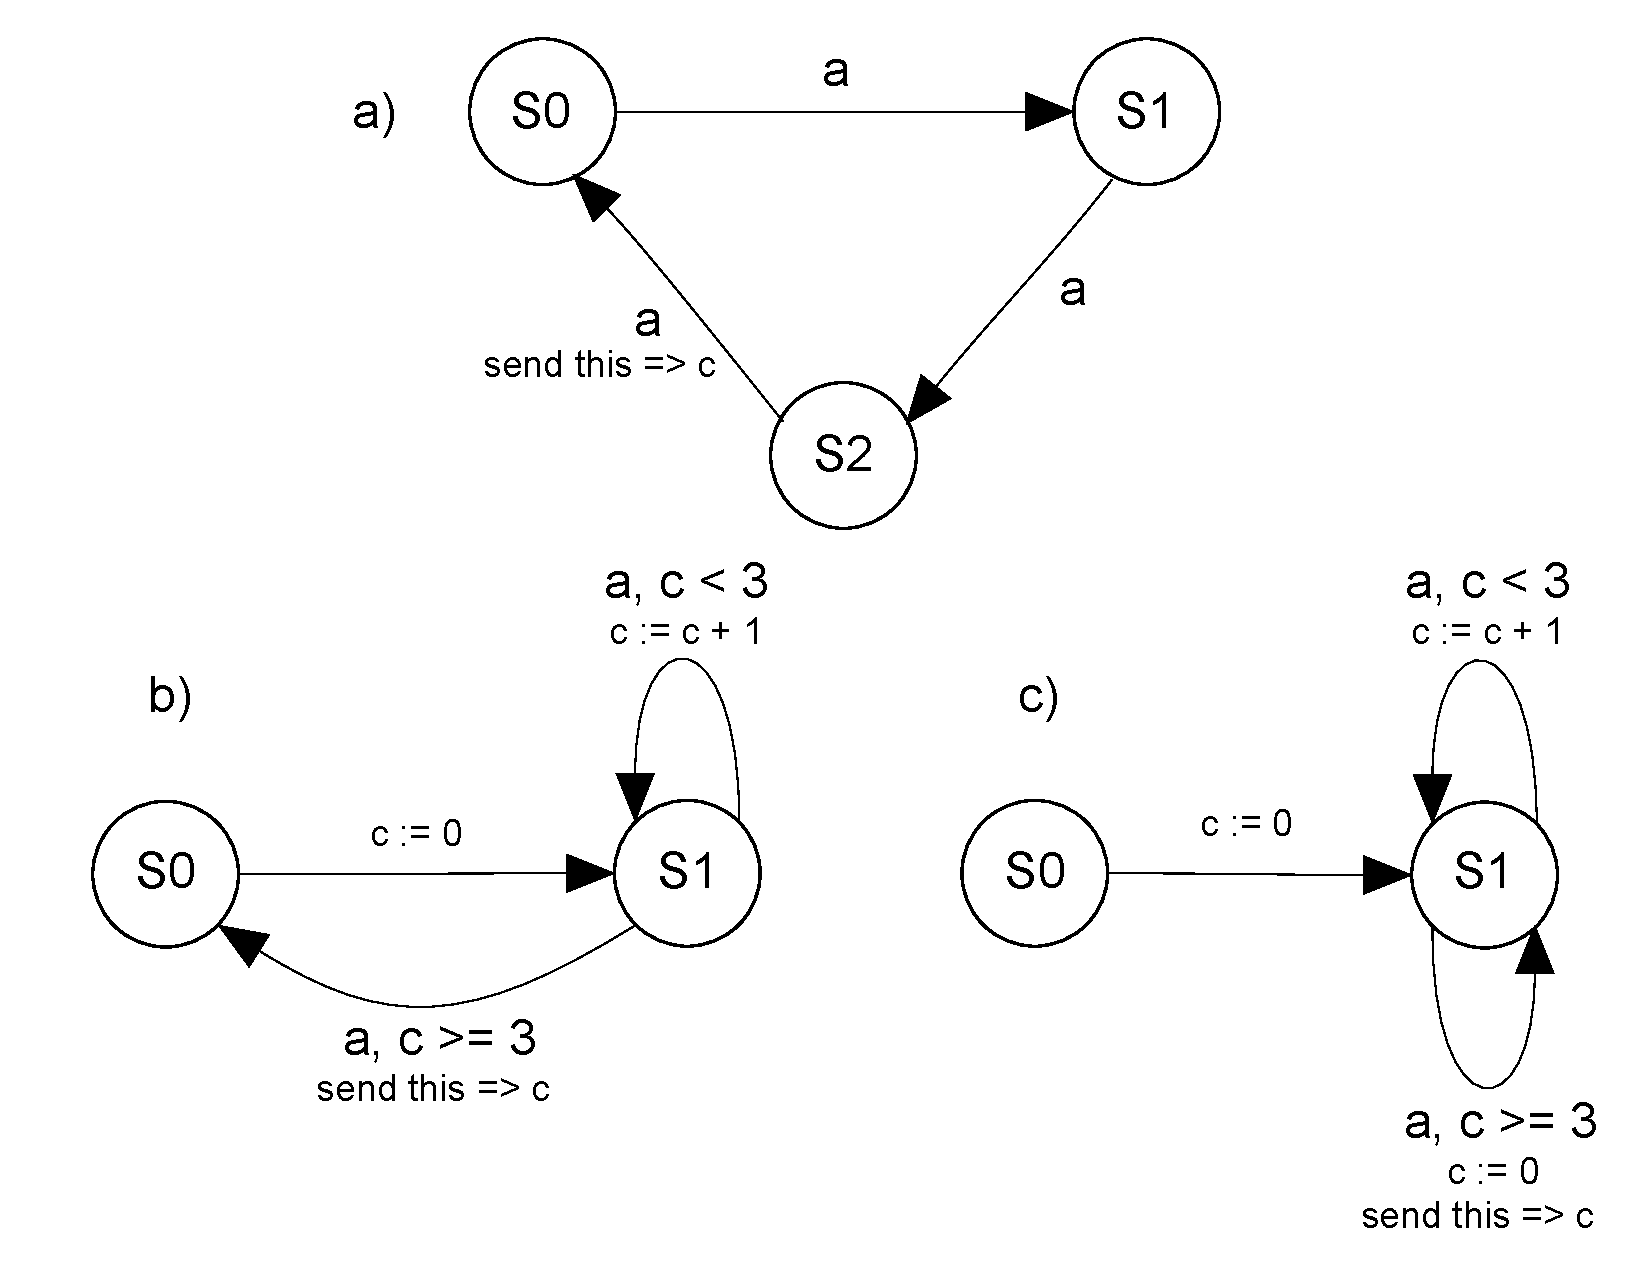
\includegraphics[scale=0.4]{figs/counter.pdf}
  \caption{The transition diagrams of the counter synchroniser.}
  \label{fig:counter}
  \end{figure}


  \item The selection predicate $\rho$

In a given state $k$ for each output channel $\omega_{m}$ we note all $i$ on which $\rho_{ki}^{m}$ is true. Those message values must be stored in a previous state and recalled in state $k$. It is expected that the boolean vector $\omega_{i} = \rho_{ki}^{m}$ has only very few true elements.

Consequently the storage mechanism that \ak\ provides for synchronisers is in the form of individual \emph{store} variables. The type of a store variable is determined when a variable is assigned.

\textbf{Example: the binary zip synchroniser}  Zip2 receives messages on its input channels and sends their concatenation to the output channel. In the resulting concatenation there's exactly one message from each input channel and those messages are ordered as they received.

The zip2 transition diagram is given in Figure \ref{fig:zip2}. The message received in the current transition is referred by a keyword \emph{this}. $ma$ and $mb$ are the store variables associated with the input channels $a$ and $b$ respectively. The statement \emph{send} indicates a sending of a message to an output channel.

  \begin{figure}[here]
  \centering
  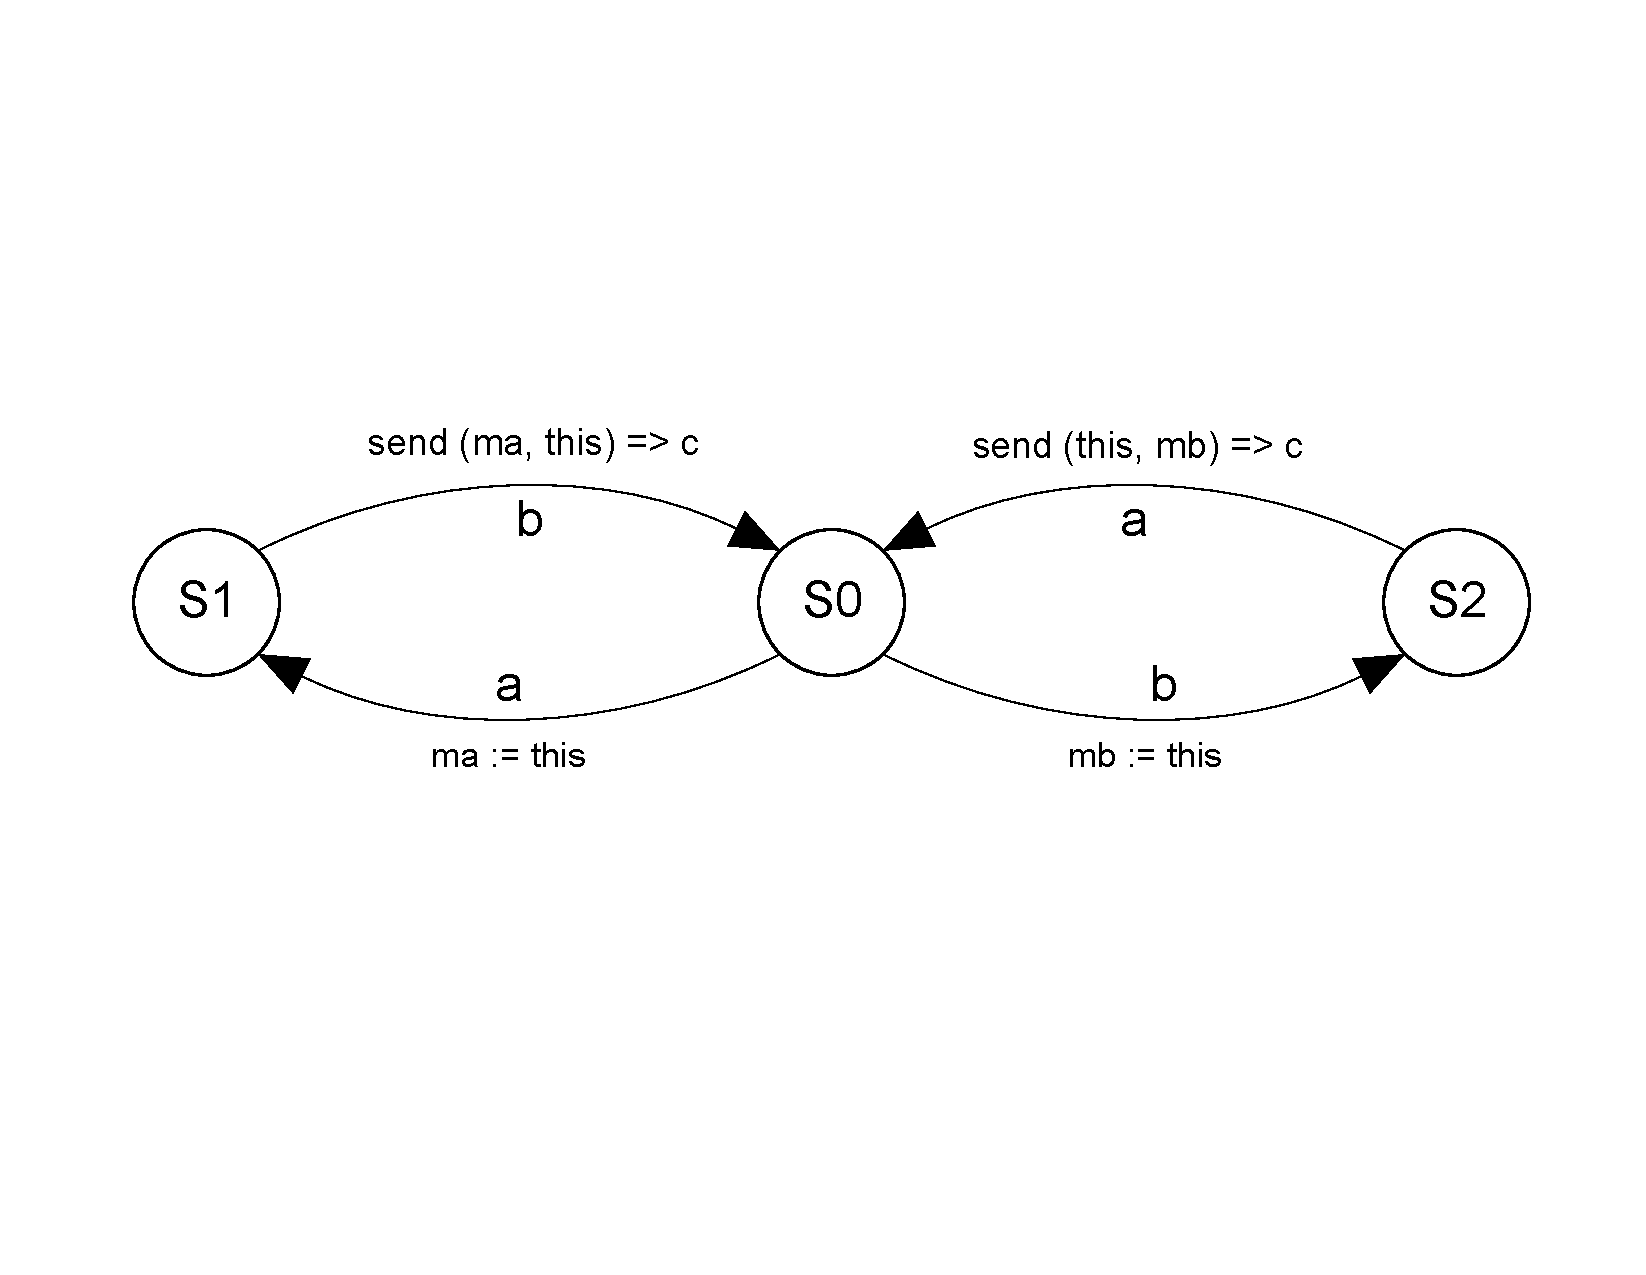
\includegraphics[scale=0.4]{figs/zip2.pdf}
  \caption{The transition diagram of the zip2 synchroniser.}
  \label{fig:zip2}
  \end{figure}

Mathematical model $S_{zip2} = (\Phi, \; \Pi)$, where
  \begin{itemize}
  \item[] $\Phi = (A, \; S, \; T)$,
    \begin{itemize}
    \item[] $C = (a, \; b)$, $P = (true)$, $A = C \times P = ((a, \; true), \: (b, \; true))$,
    \item[] $S = (s_{0}, s_{1}, s_{2})$, $s_{0}$ -- start state,
    \item[] $T$:
      \begin{tabular}{c|c|c|c}
      $A$ \textbackslash $S$ & $s_{0}$ & $s_{1}$ & $s_{2}$\\
      \hline
      $(a, \; true)$ & $s_{1}$ & $s_{1}$ & $s_{0}$\\
      \hline
      $(b, \; true)$ & $s_{2}$ & $s_{0}$ & $s_{2}$\\
      \end{tabular}
    \end{itemize}
  \item[] $\Pi \: : \: S \times \Omega \to V$,
    \begin{itemize}
    \item[] $\Omega = (c)$,
    \item[] $V = ((a, \; b), \: (b, \; a))$
    \end{itemize}
  \end{itemize}

An output message is emitted when a transition happens either from the state $s_{1}$ or the state $s_{2}$. These states are reached in two paths:
  \begin{itemize}
  \item[]
$W_{0} = ((s_{0}, \; a), \: (s_{1}, \; b))$

$\Pi \; (s_{1}, c) = \psi_{\sqcap} \; \{\mu_{0} = a \: | \: \rho_{10}^{c} \; (s_{0}) = 1, \mu_{1} = b \: | \: \rho_{11}^{c} \; (s_{1}) = 1\}$, $k = 1$, $i = 0,1$
  \item[]
$W_{1} = ((s_{0}, \; b), \: (s_{2}, \; a))$

$\Pi \; (s_{2}, c) = \psi_{\sqcap} \; \{\mu_{0} = b \: | \: \rho_{20}^{c} \; (s_{0}) = 1, \mu_{2} = a \: | \: \rho_{22}^{c} \; (s_{2}) = 1\}$, $k = 2$, $i = 0,2$ 
  \end{itemize}
  \end{enumerate}


\section{Synchroniser code}
An \ak\ synchroniser is a finite state machine, therefore the basic building blocks of a synchroniser program are states and transitions. A state of a synchroniser is fully defined by the corresponding state of the finite state machine and the values of the state variables. A transition is the act of moving to another state which is initiated by a triggering event. A triggering event for the synchroniser transition is an arrival of a message to the associated channel. The message may be required to have a specific structure. In addition, a transition may be guarded by special conditions on the values of the state variables. If the conditions are satisfied the transition fires, otherwise it is cancelled.

Once a transition is known to fire, optional actions may be performed before the underlying state machine makes the move. These actions include changing the state and store variable values and sending messages to the output channels. In order to change the state and store variables, the synchroniser language provides state and store expressions over them.

This section gives an overview of the \ak\ synchroniser programming language. The formal grammar of the \ak\ synchroniser is provided in Appendix \ref{sync_syntax}.

  \subsection{Program structure}
A synchroniser program consists of a header followed by the synchroniser's body wrapped in braces. The begining of a synchroniser program is indicated by the keyword $sync$.

The header of a synchroniser program contains the synchroniser's name and the channel signature. The name is an ASCII string that follows the C convention.

The body of the synchroniser lists the state and store variables declarations and the states of the underlying finite state machine. Each state is defined by a list of transitions. Each transition lists its triggering condition which includes an optional guarding state expression, an optional list of actions, and, finally, the destination state.

%  \subsection{Macros}
%%%
%%% We removed macros from the language. The compiler must invoke a preprocessor to expand them.
%%%
%The synchroniser language provides macros to avoid having to trivially alter synchroniser programs. Macros are specified in brackets between the synchroniser's name and its channel signature. An example of a configurable synchroniser can be found in \cite{astrakahn}.

  \subsection{Channel signature}
The channel signature defines the input channels and the output channels of the synchroniser and their bracketing depths. The synchroniser header (Fig. \ref{min_sync_head}) declares the synchroniser $min$ with two input channels that are connected to the ports $a$, $b$ and two output channels that are connected to the ports $c$, $d$. If the bracketing depths of the channels are not specified, they are assumed to be 0. Thus, the bracketing depth of the channel $a$ is 0.

The input channel depth $-1$ indicates that the input channel is ignored in the synchroniser program. The output channel with the depth $-1$ must not have data sent to them.

\begin{figure}[h!]
\begin{lstlisting}[frame=single]
sync min (a, b:p | c:2, d:p+1)
\end{lstlisting}
\caption{The synchroniser header}
\label{min_sync_head}
\end{figure}

The \ak\ synchroniser allows to declare constant and configurable integer depths for the input and output channels. In addition, the depth of the output channel can be specified with an integer shift to the configurable input channel depth.

The input channels are required to have the bracketing depths specified in the signature. Thus, the channel connected to the port $a$ of the $min$ synchroniser must have zero bracketing depth. The channel connected to the port $b$ has a configurable bracketing depth $p$. Actual values of configurable bracketing depths of input channels are determined by the \ak\ compiler. Once defined in the signature, configurable bracketing depths may be used in state expressions. They are interpreted as read-only state variables.

The output channels of a synchroniser are guaranteed to have the bracketing depths specified in the channel signature. Thus, the synchroniser $min$ must send messages to the output channel connected to the port $c$ at the depth 2 and optionally at the depths $0$, $1$. The output channel connected to the port $d$ must have the bracketing depth $p+1$ that is the depth of the input channel connected to the port $b$ shifted by $1$.



  \subsection{Variable declaration}
All the state and store variables are global to all the synchroniser transitions.


  \subsection{States and transitions}
Transitions of the synchroniser define which channels are read and in what order. The on-clause defines the condition on which the transition takes place. The do-clause is a list of actions that evaluate the functional. The send-clause forms and sends the output messages. The goto-clause defines the state transition.

Whether a transition takes place depends on the channel status and optionally the content of the messages. The state transitions of a synchroniser can depend on the content of the current message but never on that of a stored one.

The channel name $\langle$chan$\rangle$ on its own stands for the availability predicate for the corresponding channel, i.e. the condition that a message of any kind is available.

The condition $\langle$chan$\rangle$\begin{bf}.else\end{bf} is equivalent to $\langle$chan$\rangle$ except it is tested after any other condition involving the channel. Although several different channels can be tested in any given state, once a test has established the readiness of a channel, the synchroniser is committed, hence the set of conditions applied to the message on any input channel $\langle$chan$\rangle$ must be exhaustive. If it is not, the final clause \begin{bf}on\end{bf} $\langle$chan$\rangle$\begin{bf}.else;\end{bf} is assumed. That clause discards the input message and transitions the synchroniser back to its current state.

A channel carries a stream that consists of messages and possibly segmentation marks. The synchroniser detects a segmentation mark of the depth $\langle$id$\rangle$ with the channel condition \begin{bf}on\end{bf} $\langle$chan$\rangle${\tt .@}$\langle$id$\rangle$. 

When a message is received on a channel, it can be matched with a pattern $\langle$pattern$\rangle$ in order to extract parameters needed to select a specific transition. (TODO: what is a tail and how is it used?) To support message formats where several variants of a message are possible, a qualifier \begin{bf}?\end{bf}$\langle$id$\rangle$ is available as an input condition. It qualifies input messages as belonging to the $\langle$id$\rangle$ variant.

(TODO: how does elseon-clause behave?)

The synchroniser functional is evaluated with the action list that is specified within the do-clause.

Non-terminal symbol $\langle$int-exp$\rangle$ stands for integer expressions. The grammar for integer expression used in our implementation of a synchroniser compiler (Appendix \ref{int_exp_gr}) is a simplified version of the C grammar for arithmetic expression. Integer experessions can be assigned to state variables and to undeclared variables that are considered aliases for integer expressions. Such variables are used only within the transition where they were activated.

(TODO: check it) Data expression combine messages, message tails and store variables. Parentheses denote the concatenation of the messages between them.

(TODO: fix) In an array of synchronisers replicas may include an explicit $\langle$id$\rangle$$=$$\langle$integer$\rangle$ pair into an output message. This would result in the output message being inserted in another replica's output sequence non-deterministically.

A message received on a channel is referred to by the keyword 'this' within the active transition.

Messages are formed and sent to the output channels using the send-clause. Messages are dispatched 


  \subsection{Keywords, reserved words and punctuation}
The keywords, the reserved words and the punctuation used in the \ak\ synchroniser sytax are shown in Fig. \ref{sync_kw}.
\begin{figure}
\centering
\begin{tabular}{|c|p{0.7\textwidth}|}
\hline
Keywords & sync, store, state, int, enum, on, elseon, else, do, send, goto\\
\hline
Reserved words & nil, this\\
\hline
Punctuation & braces, brackets, parantheses, the comma, the dot, the semicolon, the plus sign, the minus sign, the ampersand, the at sign, the question mark, the bar-bar sign, the equality sign, the arrow\\
\hline
\end{tabular}
\caption{\ak\ synchroniser keywords, reserved words and punctiation}
\label{sync_kw}
\end{figure}
 
%%%%%%
A user-defined identifier is an ASCII string that follows the C conventions.


\section{Execution order of synchroniser\label{execod}}
Fairness policy
?on-elseon priorities
Algorithm of the execution of synchronisers, in which order transitions execute


\section{The implementation of the compiler}
The implementation of the compiler frontend in OCaml \cite{realworldocaml}, with code generation to a python structure.

  \subsection{Type checking}
  \subsection{Synchroniser passport}
%  \subsection{Dead code elimination}
%Based on Section \ref{execod}.
